\documentclass[11pt,a4paper]{article}

% --- Packages ---
\usepackage[utf8]{inputenc}
\usepackage[margin=1in]{geometry}
\usepackage{amsmath,amssymb}
\usepackage{graphicx}
\usepackage{booktabs}
\usepackage{listings}
\usepackage{xcolor}
\usepackage{fancyhdr}
\usepackage{microtype}
\usepackage{tikz}
\usetikzlibrary{arrows.meta, positioning, shapes.geometric, calc}

% --- Hyperref Setup ---
\usepackage{hyperref}
\hypersetup{
    colorlinks=true,
    linkcolor=blue,
    citecolor=red,
    urlcolor=teal,
    pdftitle={MeetFlow - Phase 1 Implementation Plan},
    pdfauthor={MeetFlow Engineering Team}
}
\usepackage{cleveref}

% --- Custom Page Layout ---
\pagestyle{fancy}
\fancyhf{}
\setlength{\headheight}{14.5pt}
\rhead{\textbf{MeetFlow Phase 1 Plan}}
\lhead{One-to-One WebRTC Baseline}
\rfoot{Page \thepage}
\lfoot{Internal Development Roadmap}
\renewcommand{\headrulewidth}{0.4pt}
\renewcommand{\footrulewidth}{0.4pt}

% --- Code Block Style ---
\definecolor{codegray}{rgb}{0.96,0.96,0.96}
\definecolor{codeblue}{rgb}{0.1,0.2,0.6}
\definecolor{codegreen}{rgb}{0.1,0.5,0.1}

\lstset{
    backgroundcolor=\color{codegray},
    basicstyle=\small\ttfamily,
    breakatwhitespace=false,
    breaklines=true,
    captionpos=b,
    commentstyle=\color{codegreen},
    keywordstyle=\color{codeblue},
    numbers=left,
    numberstyle=\tiny\color{gray},
    numbersep=5pt,
    showspaces=false,
    showstringspaces=false,
    showtabs=false,
    tabsize=2,
    frame=single,
    rulecolor=\color{lightgray}
}

\lstdefinelanguage{json}{
    stringstyle=\color{codeblue},
    string=[s]{"}{"},
    comment=[l]{//},
    morecomment=[s]{/*}{*/},
}

% --- Document Info ---
\title{
    \vspace{1.5in}
    \Huge \textbf{MeetFlow} \\
    \Large Phase 1 Implementation Plan \\
    \vspace{0.3in}
    \huge \textbf{One-to-One P2P Video Baseline} \\
    \large Detailed Task Division \& Startup Guide for a 2-Member Team
    \vspace{1.5in}
}
\author{
    \textbf{MeetFlow Engineering Team}
}
\date{\today}

\begin{document}

\maketitle
\thispagestyle{empty}
\newpage

\tableofcontents
\newpage

% =========================================================================
\section{Executive Summary}
% =========================================================================
This document details the development roadmap and role assignment for executing \textbf{Phase 1 (One-to-One Baseline)} of the MeetFlow project. 

The primary objectives of Phase 1 are:
\begin{itemize}
    \item Establish a robust Client-Server Socket.IO signaling connection.
    \item Implement dynamic room creation and joining APIs.
    \item Set up the WebRTC \texttt{RTCPeerConnection} lifecycle to negotiate and stream peer-to-peer audio and video directly between two browsers.
\end{itemize}

This guide divides tasks for a \textbf{two-member engineering team} (referred to as \textbf{Engineer A: Backend \& Infrastructure} and \textbf{Engineer B: Frontend \& WebRTC Client}).

% =========================================================================
\section{Team Roles \& Responsibility Matrix}
% =========================================================================
To complete Phase 1 efficiently, development is split into parallel paths, converging during integration and testing.

\subsection{Engineer A: Backend \& Infrastructure}
Engineer A is responsible for the foundation server, room management logic, and the WebSocket signaling gateway.
\begin{itemize}
    \item \textbf{Tech Stack Focus:} Node.js, Express, Socket.IO, CORS configuration.
    \item \textbf{Key Tasks:}
    \begin{enumerate}
        \item Set up the Node.js development server with environment configurations.
        \item Create HTTP endpoints to generate and validate unique Room IDs.
        \item Implement the Socket.IO server to orchestrate signaling events (\texttt{join-room}, relaying \texttt{offer}, \texttt{answer}, and \texttt{ice-candidate}).
        \item Manage transient room states (e.g., tracking socket IDs of participants per room).
    \end{enumerate}
\end{itemize}

\subsection{Engineer B: Frontend \& WebRTC Client}
Engineer B is responsible for the user interface, media device acquisition, socket connection client, and WebRTC peer connection management.
\begin{itemize}
    \item \textbf{Tech Stack Focus:} React, Vite, Socket.IO-Client, WebRTC API.
    \item \textbf{Key Tasks:}
    \begin{enumerate}
        \item Bootstrap the React + Vite application and set up basic routing/views.
        \item Build the UI forms to create a new meeting room or join an existing one.
        \item Implement local camera and microphone stream capture via \texttt{navigator.mediaDevices.getUserMedia()}.
        \item Orchestrate the \texttt{RTCPeerConnection} state machine (handling track additions, local/remote description configuration, and ICE candidates).
        \item Design the media stage grid displaying the local and remote HTML video elements.
    \end{enumerate}
\end{itemize}

\subsection{Collaborative Milestones}
Both engineers must pair-program on the following critical integration steps:
\begin{itemize}
    \item **Signaling Contract Definition:** Agreeing on exact Socket.IO event names and JSON payload schemas.
    \item **End-to-End P2P Negotiation:** Debugging the SDP offer/answer handshakes and ICE candidate exchange.
    \item **Local Network Testing:** Conducting multi-device tests (e.g., phone to laptop, or two browser tabs) on the same local area network (LAN).
\end{itemize}

\newpage

% =========================================================================
\section{Step-by-Step Startup Guide}
% =========================================================================

\subsection{Step 1: Preamble \& Agreement on the Signaling Protocol (Both Engineers)}
Before writing any code, both engineers must finalize the signaling protocol contract. The standard exchange pattern is diagrammed below:

\begin{figure}[h!]
\centering
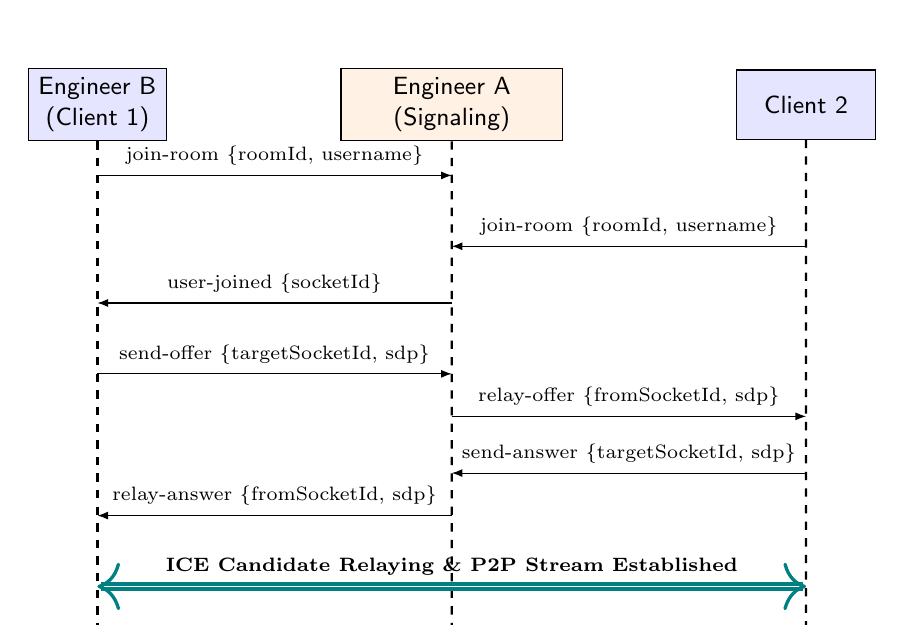
\begin{tikzpicture}[
    scale=0.9,
    every node/.style={font=\small\sffamily},
    actor/.style={draw, fill=blue!10, rectangle, minimum height=2.5em, minimum width=5em, align=center},
    server/.style={draw, fill=orange!10, rectangle, minimum height=2.5em, minimum width=8em, align=center}
]
    % Lifelines
    \node[actor] (A) at (0, 0) {Engineer B\\(Client 1)};
    \node[server] (S) at (5, 0) {Engineer A\\(Signaling)};
    \node[actor] (B) at (10, 0) {Client 2};
    
    \draw[dashed, thick] (A) -- (0, -7.5);
    \draw[dashed, thick] (S) -- (5, -7.5);
    \draw[dashed, thick] (B) -- (10, -7.5);

    % Protocol Actions
    \draw[-{Latex[scale=0.8]}] (0, -1) -- (5, -1) node[midway, above, font=\scriptsize] {join-room \{roomId, username\}};
    \draw[-{Latex[scale=0.8]}] (10, -2) -- (5, -2) node[midway, above, font=\scriptsize] {join-room \{roomId, username\}};
    \draw[-{Latex[scale=0.8]}] (5, -2.8) -- (0, -2.8) node[midway, above, font=\scriptsize] {user-joined \{socketId\}};
    
    \draw[-{Latex[scale=0.8]}] (0, -3.8) -- (5, -3.8) node[midway, above, font=\scriptsize] {send-offer \{targetSocketId, sdp\}};
    \draw[-{Latex[scale=0.8]}] (5, -4.4) -- (10, -4.4) node[midway, above, font=\scriptsize] {relay-offer \{fromSocketId, sdp\}};
    
    \draw[-{Latex[scale=0.8]}] (10, -5.2) -- (5, -5.2) node[midway, above, font=\scriptsize] {send-answer \{targetSocketId, sdp\}};
    \draw[-{Latex[scale=0.8]}] (5, -5.8) -- (0, -5.8) node[midway, above, font=\scriptsize] {relay-answer \{fromSocketId, sdp\}};
    
    \draw[<->, double, color=teal, line width=1.2pt] (0, -6.8) -- (10, -6.8) node[midway, above, font=\scriptsize\bfseries, color=black] {ICE Candidate Relaying \& P2P Stream Established};
\end{tikzpicture}
\caption{Phase 1 Signaling and Connection Protocol}
\label{fig:phase1_flow}
\end{figure}

\subsection{Step 2: Backend Core Setup (Engineer A)}
Engineer A initiates the workspace backend folder structure:
\begin{lstlisting}[language=bash]
mkdir server
cd server
npm init -y
npm install express socket.io cors dotenv
\end{lstlisting}
Configure an \texttt{index.js} that boots an HTTP server listening on port \texttt{5000} and binds Socket.IO with CORS settings allowing traffic from the frontend development port (typically \texttt{http://localhost:5173}).

\subsection{Step 3: Frontend Client Setup (Engineer B)}
Engineer B bootstraps the client folder layout in parallel:
\begin{lstlisting}[language=bash]
npm create vite@latest client -- --template react
cd client
npm install socket.io-client react-router-dom lucide-react
\end{lstlisting}
Design the routing layout using React Router:
\begin{itemize}
    \item \texttt{/} $\rightarrow$ Landing Screen (Join Room form / Create Room button).
    \item \texttt{/room/:roomId} $\rightarrow$ Video Conference Room.
\end{itemize}

\newpage

% =========================================================================
\section{Detailed Task Breakdown \& Timeline}
% =========================================================================

\begin{table}[h!]
\centering
\begin{tabular}{@{}llp{8cm}@{}}
\toprule
\textbf{Day} & \textbf{Assignee} & \textbf{Task Description} \\ \midrule
\textbf{Day 1} & Eng A & Setup basic Express app, configure environmental variables, and build a REST API (\texttt{POST /api/rooms}) returning a unique 9-digit hyphenated Room ID (\texttt{XXX-XXX-XXX}). \\
& Eng B & Create frontend boilerplate with routing. Design the landing page containing a text input for Room ID, user nickname, and buttons. \\ \midrule
\textbf{Day 2} & Eng A & Initialize Socket.IO connection handlers. Write room state management to prevent more than two users from joining the same room (One-to-One boundary). \\
& Eng B & Add camera and microphone selection logic. Render the local camera track onto a \texttt{<video>} component with audio muted locally to prevent feedback. \\ \midrule
\textbf{Day 3} & Eng A & Complete signaling event listeners (\texttt{offer}, \texttt{answer}, \texttt{ice-candidate}) that target a specific peer socket. \\
& Eng B & Build the Socket manager in React using React contexts or custom hooks. Verify connection states, connect client sockets, and join the correct room. \\ \midrule
\textbf{Day 4} & Both & **Integration Day 1**: Link frontend client sockets to the backend. Verify logging on server when a user enters/leaves, and check user count limits. \\ \midrule
\textbf{Day 5} & Eng B & Write the WebRTC core handshake: Instantiate \texttt{RTCPeerConnection}, attach media tracks, capture generated local ICE candidates, and trigger SDP offer generation upon receiving \texttt{user-joined}. \\
& Eng A & Assist with real-time logging, testing websocket packet integrity, and configuring fallback STUN servers. \\ \midrule
\textbf{Day 6} & Both & **Integration Day 2**: Verify the complete WebRTC handshake. Configure the remote stream component, bind incoming tracks to the \texttt{remoteVideo} HTML element, and test audio/video flow. \\ \midrule
\textbf{Day 7} & Both & Perform local loopback tests, verify NAT traversal on different browser engines (Chrome vs Firefox/Safari), and package codebase for Phase 2. \\ \bottomrule
\end{tabular}
\caption{Phase 1 Action Schedule}
\label{tab:schedule}
\end{table}

% =========================================================================
\section{Signaling Server Interface Contract}
% =========================================================================
To prevent runtime configuration disparities, the Socket.IO communication must adhere to these exact structures:

\subsection{Client Emit: Join Room}
Emitted by the client immediately upon mounting the room page.
\begin{lstlisting}[language=json]
{
  "roomId": "abc-123-xyz",
  "username": "EngineerB"
}
\end{lstlisting}

\subsection{Server Broadcast: User Joined}
Broadcasted by the server to the existing socket in the room when a second peer joins.
\begin{lstlisting}[language=json]
{
  "socketId": "socket_id_of_new_peer",
  "username": "EngineerB"
}
\end{lstlisting}

\subsection{Client Emit: SDP Negotiation (Offer / Answer)}
Clients wrap descriptions in these formats before sending them to the signaling relay:
\begin{lstlisting}[language=json]
{
  "targetSocketId": "socket_id_of_recipient",
  "sdp": {
    "type": "offer", // or "answer"
    "sdp": "v=0\r\no=- 52362354256..."
  }
}
\end{lstlisting}

\subsection{Client Emit: ICE Candidate}
Clients must package network paths immediately upon discovery:
\begin{lstlisting}[language=json]
{
  "targetSocketId": "socket_id_of_recipient",
  "candidate": {
    "candidate": "candidate:842163049 1 udp 1686052607 192.168.1.100...",
    "sdpMid": "0",
    "sdpMLineIndex": 0
  }
}
\end{lstlisting}

\newpage

% =========================================================================
\section{Testing, Diagnostics \& Debugging Tips}
% =========================================================================

To resolve WebRTC issues quickly during development, follow these standard diagnostic procedures:

\subsection{Recommended WebRTC Debugging Tools}
\begin{itemize}
    \item \textbf{Chrome Internal Page:} Access \texttt{chrome://webrtc-internals/} in your browser tab during an active session. It provides real-time graphs showing bytes sent/received, connection states, and ICE selection processes.
    \item \textbf{Firefox WebRTC Tooling:} Navigate to \texttt{about:webrtc} for connection logs.
\end{itemize}

\subsection{Common Gotchas \& Solutions}
\begin{enumerate}
    \item \textbf{No Audio/Video Flowing:} Check if the browser block settings are active. WebRTC requires secure origins. Use \texttt{http://localhost} for local testing; if testing over a local network, configure the backend and frontend servers on HTTPS, or bypass browser policies in Chrome via:
    \texttt{chrome://flags/\#unsafely-treat-insecure-origin-as-secure}.
    \item \textbf{ICE Connection Fails:} Ensure you use public STUN servers in your client setup. A free, public server like \texttt{stun:stun.l.google.com:19302} must be supplied in your \texttt{RTCConfiguration} object:
\begin{lstlisting}
const peerConnection = new RTCPeerConnection({
  iceServers: [
    { urls: 'stun:stun.l.google.com:19302' }
  ]
});
\end{lstlisting}
    \item \textbf{Local Audio Feedback:} Ensure the local HTML \texttt{<video>} element has the \texttt{muted} attribute enabled. Do not mute the remote video stream.
\end{enumerate}

\end{document}
